\section{Возобновление связи}\label{COMMON.Resume} 

Секрет режима PSK может быть согласован как за пределами TLS, так и в 
самом протоколе. В последнем случае секрет является одним из общих ключей, 
формируемых в сеансе Handshake. Клиент и сервер используют секрет в следующих 
сеансах протокола, возобновляя уже налаженную защищенную связь друг с другом. 
При возобновлении связи стороны используют ранее согласованные параметры и 
ключи, ускоряя выполнение Handshake.

Для возобновления связи сервер по завершении Handshake направляет клиенту
сообщение~\token[HS.NST]{NewSessionTicket}, в котором указывает
идентификатор сформированного секрета.
%
Клиент сохраняет секрет вместе с присланным идентификатором. Клиент может
хранить несколько секретов, полученных по завершении различных сеансов
Handshake.
%
В~\token[HS.CH]{ClientHello} нового сеанса клиент включает
расширения~\token[HS.Ext.pkem]{psk_key_exchange_modes}
и~\token[HS.Ext.psk]{pre_shared_key}. В первом расширении клиент указывает 
допустимые для него режимы формирования общих ключей, во втором~--- 
идентификаторы сохраненных секретов.
%
Допустимыми являются режимы PSK и PSK+DHE. Последний обеспечивает защиту от 
<<чтения назад>>, т.~е. конфиденциальность переданных прикладных данных даже в  
случае компрометации секрета.

\begin{figure}[hbt]
\begin{center}
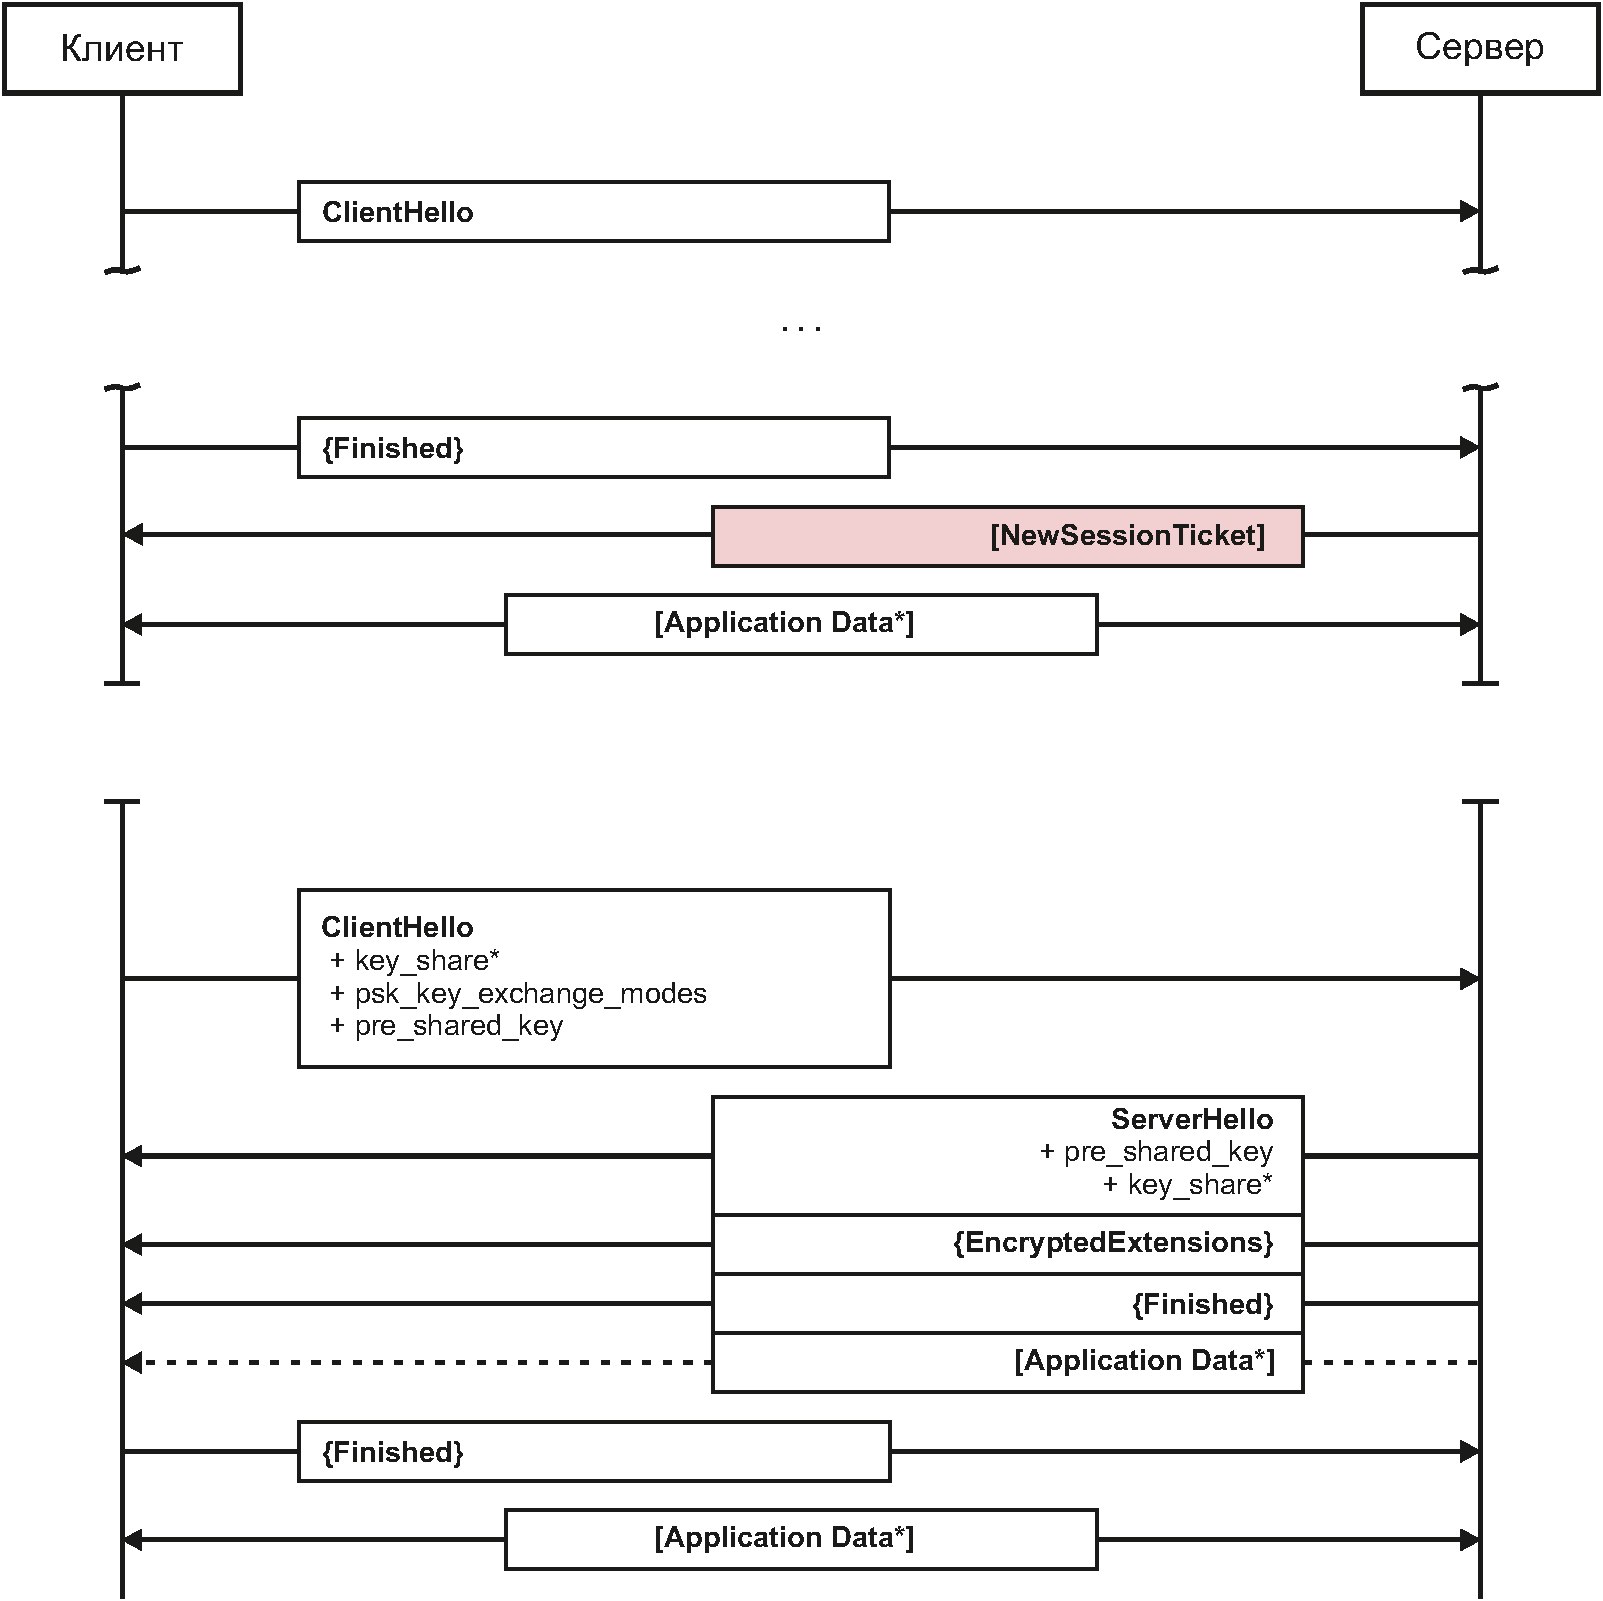
\includegraphics[width=15cm]{../figs/Resume}
\end{center}
\caption{Возобновление связи}\label{Fig.COMMON.Resume}
\end{figure}

% use: https://www.rfc-editor.org/errata/eid5717

Пример возобновления связи представлен на рисунке~\ref{Fig.COMMON.Resume}. 
В первом сеансе Handshake стороны формируют общий секрет, во втором~---
используют его. Во втором сеансе общие ключи формируются в режиме PSK и поэтому 
сервер не отправляет клиенту ни свой сертификат, ни сообщение 
\token[HS.CV]{CertificateVerify}.
%
Тем не менее, в сообщении~\token[HS.CH]{ClientHello} второго сеанса клиент может
выслать расширение~\token[HS.Ext.ks]{key_share}, допуская, что сервер откажется
от возобновления связи и будет выполнять полный Handshake.

% skip: When PSKs are provisioned out of band, the PSK identity and the KDF 
% hash algorithm to be used with the PSK MUST also be provisioned.

% skip: When using an out-of-band provisioned pre-shared secret, a critical 
% consideration is using sufficient entropy during the key generation, as 
% discussed in [RFC 4086]. Deriving a shared secret from a password or other 
% low-entropy sources is not secure. A low-entropy secret, or password, is 
% subject to dictionary attacks based on the PSK binder. The specified PSK 
% authentication is not a strong password-based authenticated key exchange even
% when used with Diffie-Hellman key establishment. Specifically, it does not 
% prevent an attacker that can observe the handshake from performing a 
% brute-force attack on the password/pre-shared key.
 